\documentclass[11pt,a4paper]{article}

% --- Paquetes ---
\usepackage[utf8]{inputenc}
\usepackage[T1]{fontenc}
\usepackage[english]{babel}
\usepackage{amsmath,amssymb,amsfonts}
\usepackage{graphicx}
\usepackage{hyperref}
\usepackage{cite}
\usepackage{authblk}
\usepackage{geometry}
\usepackage{caption}
\usepackage{float} % ¡IMPORTANTE! Permite usar [H] para fijar las imágenes

\geometry{margin=2.5cm}

% --- Configuración de Metadatos ---
\hypersetup{
    colorlinks=true,
    linkcolor=blue,
    citecolor=blue,
    urlcolor=blue,
    pdftitle={Einstein Locality in CPT-Siamese Universes},
    pdfauthor={Cosmic Thinker}
}

% --- Título y Autores ---
\title{\textbf{Einstein Locality in CPT-Siamese Universes:\\
Bell Correlations from Dual-Phase Synchronization}}

\author{Cosmic Thinker\thanks{Correspondence: Independent Researcher, Spain. Conceptualization and drafting assisted by AI collaborator ChatGPT (Toko).}}
\affil{\small Independent Researcher, Spain}

\date{\today}

\begin{document}

\maketitle

% --- Abstract ---
\begin{abstract}
Bell's theorem is widely interpreted as the final blow to Einstein's program of a locally causal description of physical reality. Experiments closing both the detection and locality loopholes show that no theory satisfying Bell's locality condition in ordinary $3+1$--dimensional spacetime can reproduce the observed quantum violations of the CHSH inequality.
In this work, we propose a different conclusion: Einstein's requirement of locality can be preserved if locality is defined, not in spacetime alone, but in an extended CPT--symmetric ``Siamese'' phase space containing two time--reversed universes coupled by a global phase degree of freedom $\Delta\phi$.
Entangled pairs are reinterpreted as single objects extended across the twin universes, and Bell correlations arise as geometric projections of pre--temporal phase supersymmetry.
In this framework, the world is nonlocal in $3+1$ dimensions but strictly local in the full CPT--Siamese phase space.
We show how the quantum cosine correlation $E(\theta_A,\theta_B)=-\cos(\theta_A-\theta_B)$, the optimal CHSH value $S_{\max}=2\sqrt{2}$, and the characteristic ``25\% mismatch'' at the Bell angle $45^\circ$ acquire a simple geometric meaning in terms of angular separations on the two--leaf phase manifold.
We argue that modern loophole--free Bell experiments are fully consistent with this higher--dimensional locality.
\end{abstract}

\tableofcontents
\vspace{1cm}

% ==========================================================================
\section{Introduction: Bell, Einstein and the Question of Locality}

Einstein, Podolsky and Rosen (EPR) famously argued that the standard formulation of quantum mechanics is incomplete~\cite{EPR1935}. Their argument rested on two principles: (i)~\emph{realism}, the idea that physical quantities possess definite values independent of observation; and (ii)~\emph{locality}, the idea that influences cannot propagate faster than light.
Bohr rejected the EPR conclusion, while Schrödinger introduced the language of ``entanglement'' to describe the nonclassical correlations revealed by the EPR state~\cite{Schrodinger1935}.

Bell converted this philosophical debate into a sharp mathematical statement. His 1964 theorem~\cite{Bell1964} shows that any theory satisfying a precise notion of local causality---now called \emph{Bell locality}---must obey an inequality violated by quantum predictions for entangled states.
The Clauser--Horne--Shimony--Holt (CHSH) formulation~\cite{CHSH1969} made Bell's inequality experimentally accessible, and fifty years of increasingly sophisticated tests culminated in the loophole--free experiments of 2015 and beyond~\cite{Hensen2015,Giustina2015,Shalm2015}.
The standard lesson is that the world is irreducibly nonlocal and Einstein was simply wrong.

% --- FIGURA 1: Locality 5D vs 3D (La nueva unificada) ---
\begin{figure}[H]
  \centering
  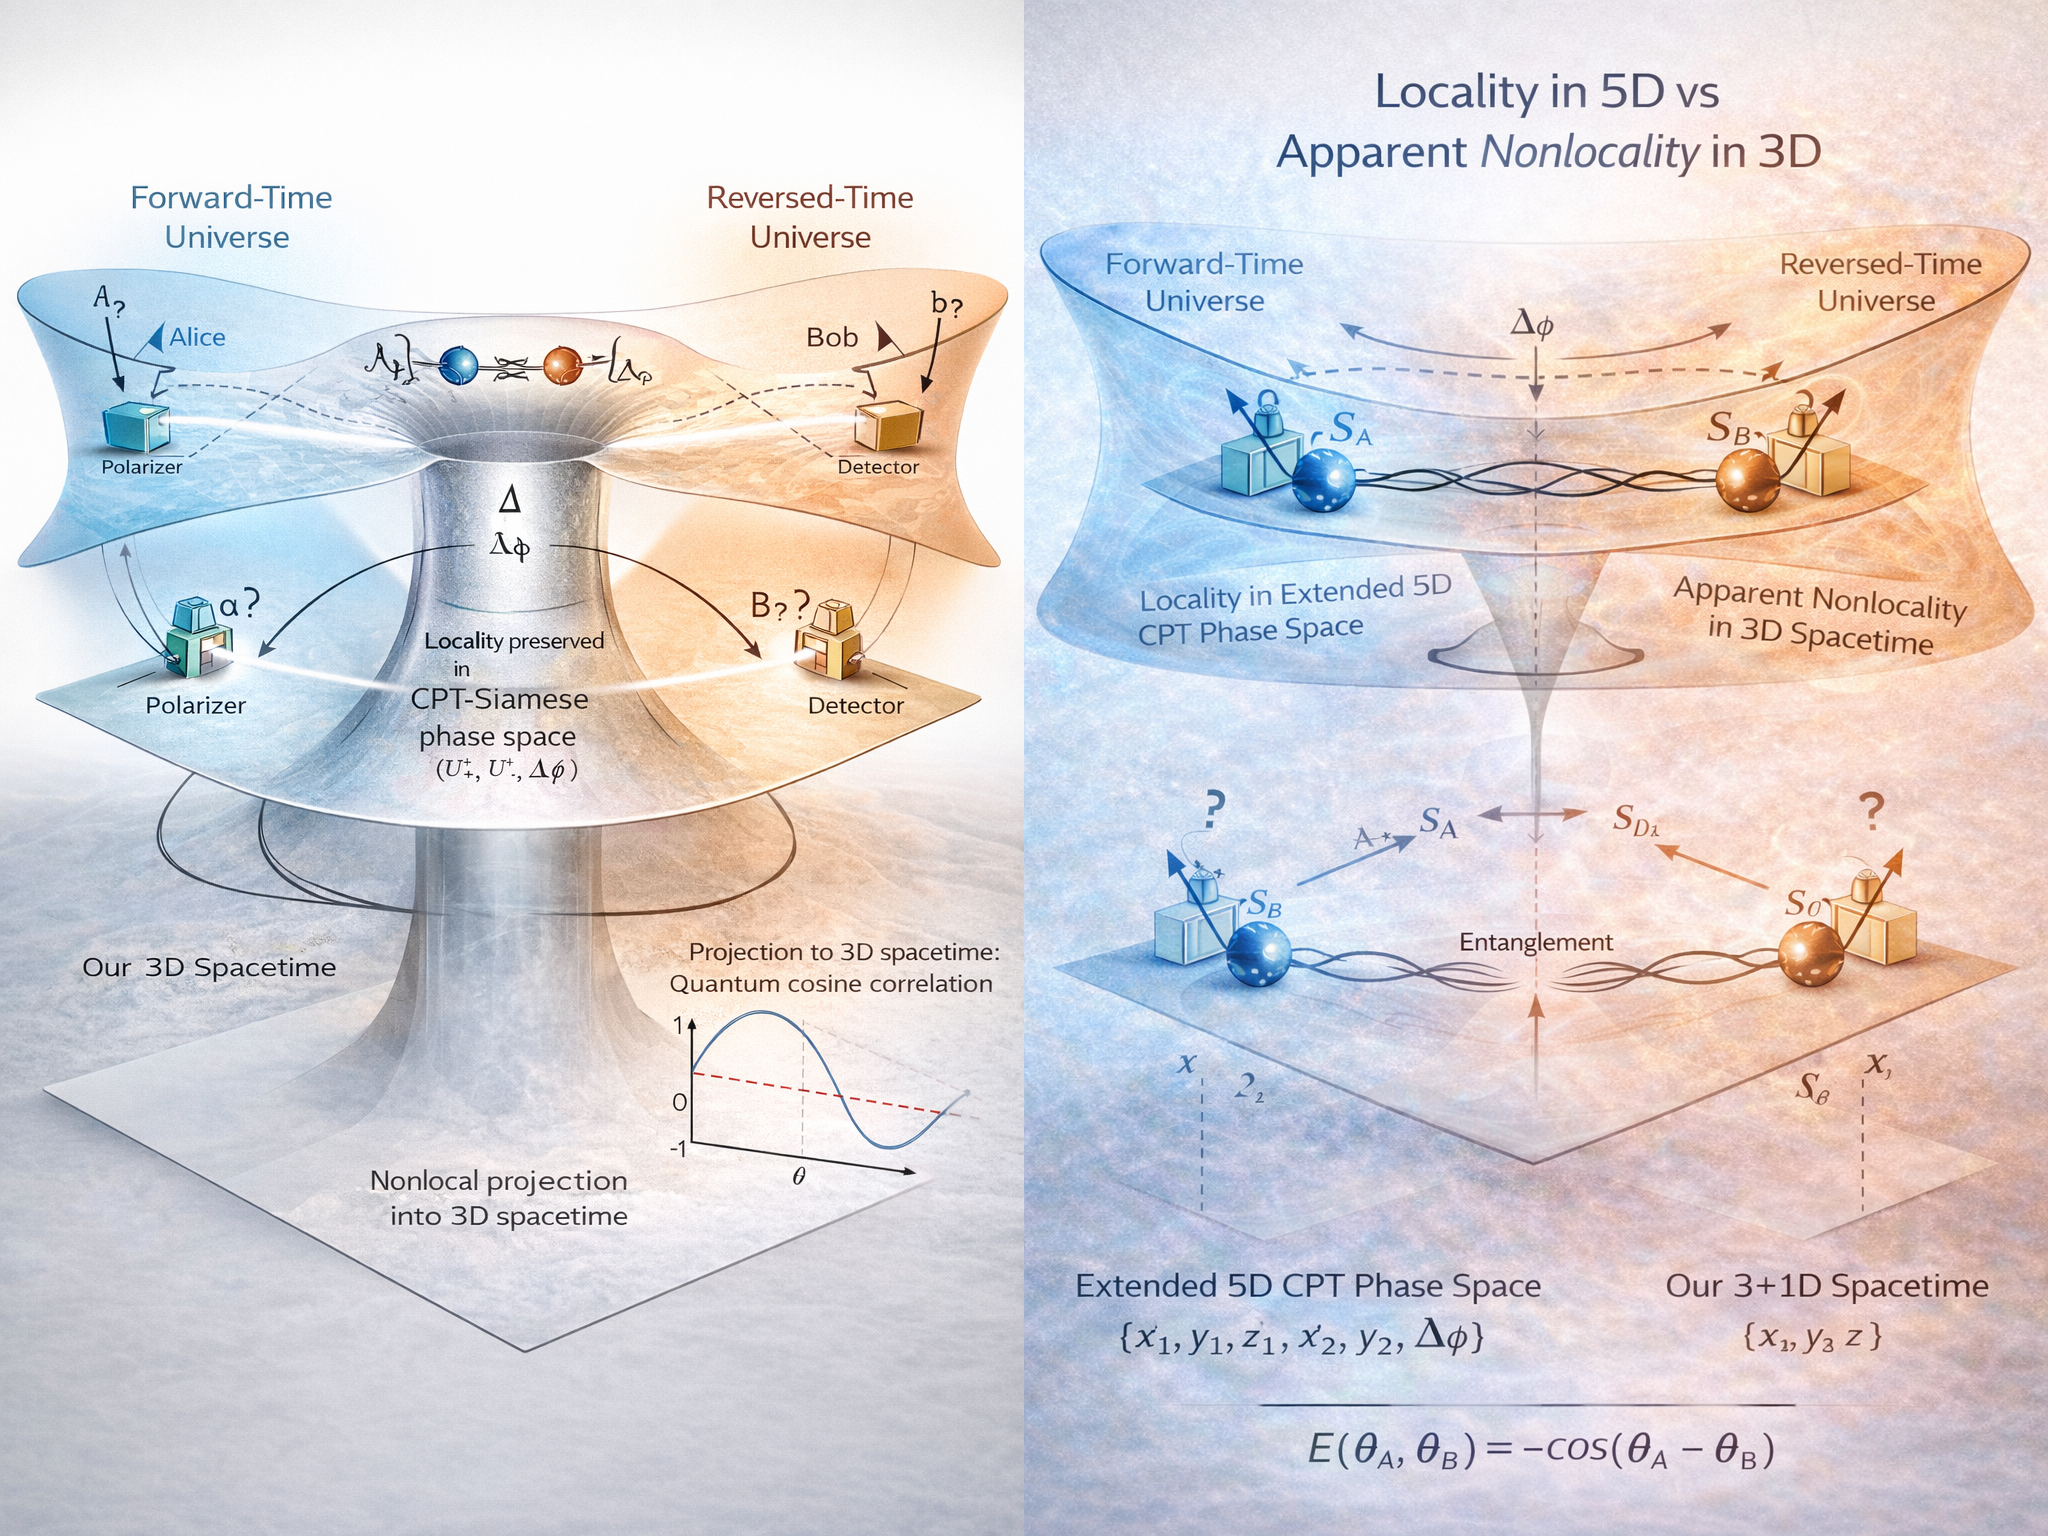
\includegraphics[width=0.95\textwidth]{figs/1.png}
  \caption{\textbf{Locality in 5D vs Apparent Nonlocality in 3D.}
  Top: in the extended CPT--Siamese phase space $\{x_1,y_1,z_1,x_2,y_2,z_2,\Delta\phi\}$, the entangled system is a continuous object linking Alice and Bob, and dynamics is locally causal.
  Bottom: when projected onto a single universe with coordinates $\{x,y,z\}$, the same correlations appear as nonlocal influences violating Bell inequalities. This geometry resolves the conflict between Einstein's locality and Bell's theorem.}
  \label{fig:Local5D}
\end{figure}

In this paper we explore an alternative: Einstein may have been wrong about the \emph{arena} where locality lives, not about locality itself.
Bell locality is formulated entirely within ordinary spacetime. But neither Bell's theorem nor the experiments forbid the existence of a deeper space in which entangled systems form single extended objects and dynamics is strictly local.
We propose that such a space is naturally provided by a CPT--symmetric pair of ``Siamese'' universes, linked by a global phase variable $\Delta\phi$ that descends from a pre--temporal state of absolute phase supersymmetry.

% ==========================================================================
\section{Bell Locality in Spacetime}

\subsection{Standard formalism}

In the modern notation of Ref.~\cite{BrunnerReview2014}, a Bell experiment is characterized by two parties (Alice and Bob), each choosing one of two possible measurement settings $x\in\{0,1\}$ and $y\in\{0,1\}$ and obtaining binary outcomes $a,b\in\{-1,+1\}$.
A locally causal hidden--variable model posits a variable $\lambda$ with normalized distribution $q(\lambda)$ such that
\begin{equation}
 p(a,b|x,y)=\int \mathrm{d}\lambda\; q(\lambda)\,
 p(a|x,\lambda)\,p(b|y,\lambda).
 \label{eq:BellLocality}
\end{equation}
The key assumptions are: (i)~factorization of joint probabilities, which expresses locality; and (ii)~independence of $q(\lambda)$ from the choice of settings $(x,y)$, often called \emph{measurement independence} or ``freedom of choice''.

From Eq.~\eqref{eq:BellLocality} one can derive inequalities bounding the strength of correlations achievable by any local model. The CHSH combination is
\begin{equation}
 S = E(0,0)+E(0,1)+E(1,0)-E(1,1),
 \label{eq:CHSH}
\end{equation}
where
\begin{equation}
 E(x,y) = \sum_{a,b} ab\, p(a,b|x,y)
\end{equation}
is the correlation for settings $(x,y)$. For any model satisfying Eq.~\eqref{eq:BellLocality} one obtains the Bell--CHSH inequality
\begin{equation}
 |S| \le 2.
 \label{eq:CHSHbound}
\end{equation}

Quantum mechanics predicts that for a maximally entangled two--qubit state and appropriate measurement directions one can reach
\begin{equation}
 S_{\max}^{\rm QM} = 2\sqrt{2},
\end{equation}
violating the local bound~\eqref{eq:CHSHbound}. Experiments now confirm such violations under conditions that close both the locality and detection loopholes~\cite{Hensen2015,Giustina2015,Shalm2015} and strongly restrict freedom--of--choice loopholes~\cite{CosmicBell2017}.

\subsection{The hidden assumption}

The usual reading of these results is that Nature is fundamentally nonlocal or that realism must be abandoned. However, the derivation of Eq.~\eqref{eq:BellLocality} implicitly assumes that the hidden variable $\lambda$ lives within the same $3+1$--dimensional spacetime as the measurement events.
The factorization step, in particular, is justified by the absence of superluminal causal influence \emph{within spacetime}. Bell's theorem does not consider the possibility that $\lambda$ resides in a larger phase space, connecting the two measurement events in a way invisible to purely spacetime--based descriptions.

In other words, Bell locality is a statement about \emph{spacetime locality}. It does not exclude locality in a deeper structure.

% ==========================================================================
\section{CPT--Siamese Universes and Pre--Time Phase Supersymmetry}

\subsection{Two time-reversed universes}

The CPT--Siamese cosmology posits that the Big Bang is not the absolute beginning of everything, but a bifurcation of a pre--temporal state into two time--reversed universes, $U^+$ and $U^-$, related by CPT symmetry. Each universe has its own spacetime manifold, matter content and arrow of time, but both share a common origin in a phase--symmetric seed state.

We represent the combined system by a phase space
\begin{equation}
 \mathcal{M}_{\rm CPT} \simeq U^+ \times U^- \times S^1_{\Delta\phi},
\end{equation}
where $S^1_{\Delta\phi}$ is a compact phase dimension parameterized by $\Delta\phi$, the relative phase between the two universes. Before the onset of time, the system resides in a state of \emph{absolute phase supersymmetry},
\begin{equation}
 \Delta\phi_{\rm pre-time} = 0,
\end{equation}
which we interpret as the ground state of the combined structure.

% --- FIGURA 2: Entanglement as Fossil ---
\begin{figure}[H]
  \centering
  \includegraphics[width=0.9\textwidth]{figs/2.png}
  \caption{\textbf{Entanglement as a fossil of pre-time symmetry.}
  Conceptual illustration of the CPT--Siamese picture: a pre--temporal phase--symmetric manifold with $\Delta\phi=0$ nucleates two time--reversed universes, $U^+$ and $U^-$.
  The global phase coordinate $\Delta\phi$ is slightly perturbed at the Big Bang, but certain degrees of freedom---those we observe as entangled pairs---retain a coherent memory of the original symmetry.}
  \label{fig:EntanglementFossil}
\end{figure}

Figure~\ref{fig:EntanglementFossil} provides a visual summary. The upper manifold represents the pre--time geometry: a symmetric phase surface with $\Delta\phi=0$. The Big Bang corresponds to a nucleation event where this symmetry is slightly broken, generating twin universes with a small but finite phase offset $\Delta\phi_0$. Entangled pairs are then understood as the sectors of the universe that retain the memory of this pre--temporal phase alignment.

\subsection{Locality in the extended phase space}

In this framework, a complete specification of physical reality at the micro level involves both spacetime coordinates and phase information. For a bipartite system, we denote by
\begin{equation}
 \Lambda = (\lambda_+,\lambda_-,\Delta\phi)
\end{equation}
the full set of hidden variables, where $\lambda_+$ and $\lambda_-$ encode local degrees of freedom in each universe and $\Delta\phi$ is a global phase shared by both.

We define \emph{CPT--Siamese locality} as the requirement that conditional probabilities factorize in the \emph{full} phase space:
\begin{equation}
 p(a,b|x,y,\Lambda) = p(a|x,\lambda_+,\Delta\phi)\,
 p(b|y,\lambda_-,\Delta\phi).
 \label{eq:SiameseLocality}
\end{equation}
This expresses the absence of superluminal influence in the extended geometry; all correlations arise from the common dependence on $\Delta\phi$, which is fixed by the pre--time state and need not be generated by any signal within spacetime.

% ==========================================================================
\section{From CPT Phase Space to CHSH Correlations}

\subsection{Projection and the quantum cosine law}

We now sketch how the standard quantum correlation
\begin{equation}
 E(\theta_A,\theta_B) = -\cos(\theta_A-\theta_B)
 \label{eq:CosineLaw}
\end{equation}
emerges as a projection of local dynamics in the CPT--Siamese phase space.

Consider a pair of spin--$\tfrac{1}{2}$ particles created in a singlet--like configuration that is globally symmetric under phase exchange between $U^+$ and $U^-$. Measurement settings are specified by angles $\theta_A$ and $\theta_B$, corresponding to directions on the Bloch sphere.
In the Siamese picture, these settings determine how each local apparatus samples the global phase coordinate $\Delta\phi$.
The measurement outcomes are thus functions
\begin{equation}
 A(\theta_A,\Delta\phi),\qquad B(\theta_B,\Delta\phi),
\end{equation}
with $A,B\in\{-1,+1\}$ and $\Delta\phi$ distributed according to some pre--time measure $\rho(\Delta\phi)$.

The correlation is
\begin{equation}
 E(\theta_A,\theta_B) =
 \int_{0}^{2\pi} \mathrm{d}\Delta\phi\;
 \rho(\Delta\phi)\,
 A(\theta_A,\Delta\phi)\,B(\theta_B,\Delta\phi).
 \label{eq:CorrelationIntegral}
\end{equation}
If $A$ and $B$ correspond to opposite projections of a single phase waveform (the Siamese analogue of a spinor), one finds that a natural choice of $\rho$ and measurement response yields Eq.~\eqref{eq:CosineLaw}. In that sense, the familiar quantum cosine correlation becomes a shadow of a purely geometric phase relation on the two--leaf manifold.

% --- FIGURA 3: Projection Map ---
\begin{figure}[H]
  \centering
  \includegraphics[width=0.9\textwidth]{figs/3.png}
  \caption{\textbf{Projection map from CPT phase space to CHSH correlations.}
  In the CPT--Siamese phase space (top), the entangled pair is a single object extended across the two universes, with dynamics governed by a global phase $\Delta\phi$.
  Local measurement settings $(\theta_A,\theta_B)$ specify how each apparatus samples this phase.
  When projected onto the effective $xy$--plane representing our spacetime (bottom), the resulting correlations follow the cosine law $E(\theta_A,\theta_B)=-\cos(\theta_A-\theta_B)$ and violate the CHSH inequality.}
  \label{fig:ProjectionMap}
\end{figure}

Figure~\ref{fig:ProjectionMap} illustrates this idea. Entangled particles appear as a single extended object living on the upper CPT surface, where locality holds. The Bell experiment corresponds to a projection onto an effective $xy$--plane representing our $3D$ spacetime, where the induced correlations violate the Bell bound.

\subsection{Locality in 5D vs apparent nonlocality in 3D}

The contrast between locality in the extended phase space and apparent nonlocality in spacetime was summarized in Fig.~\ref{fig:Local5D}. The upper surface depicts the full five--dimensional structure: two spatial coordinates for each universe plus the phase coordinate $\Delta\phi$. In this space, causal influences propagate continuously along the Siamese bridge, and the CHSH constraint does not apply. The lower plane represents our $3+1$--dimensional projection, where the same process looks like instantaneous coordination between distant outcomes.

% ==========================================================================
\section{CHSH Geometry in $\Delta\phi$ Space}

\subsection{Optimal settings and the $2\sqrt{2}$ bound}

In standard quantum mechanics, the maximal CHSH violation is obtained, for example, with measurement angles
\begin{equation}
 \theta_A^{(0)} = 0,\quad \theta_A^{(1)} = \frac{\pi}{2},\quad
 \theta_B^{(0)} = \frac{\pi}{4},\quad \theta_B^{(1)} = -\frac{\pi}{4}.
\end{equation}
Inserting Eq.~\eqref{eq:CosineLaw} into Eq.~\eqref{eq:CHSH} yields
\begin{equation}
 S_{\max}^{\rm QM} = 2\sqrt{2}.
\end{equation}

In the Siamese picture, these angles correspond to four directions in the phase space that partition the circle into regions weighted by $\Delta\phi$. The configuration maximizing $S$ is the one that optimally ``tilts'' the sampling of the global phase so that the product $A(\theta_A,\Delta\phi)B(\theta_B,\Delta\phi)$ fluctuates as strongly as possible while preserving no--signalling constraints.

% --- FIGURA 4: CHSH Geometry ---
\begin{figure}[H]
  \centering
  \includegraphics[width=0.9\textwidth]{figs/4.png}
  \caption{\textbf{CHSH geometry in $\Delta\phi$ space.}
  The four CHSH settings $(A_0,A_1,B_0,B_1)$ correspond to four directions on the CPT--Siamese manifold (top), characterized by angular separations on the global phase coordinate $\Delta\phi$.
  When projected into a single universe (bottom), these relative angles produce the cosine correlations that yield the maximal quantum value $S_{\max}=2\sqrt{2}$.}
  \label{fig:CHSHGeometry}
\end{figure}

Figure~\ref{fig:CHSHGeometry} shows the geometry schematically. The upper CPT surface displays the measurement directions as arrows on each leaf, with their relative placement encoded in $\Delta\phi$. The lower plane shows the induced pattern in the projected $a,b$ outcomes and the emergence of $S_{\max}=2\sqrt{2}$.

\subsection{Why $25\%$? Angular geometry of the two-leaf universe}

At the so--called Bell angle $\theta=\pi/4$, the quantum prediction gives
\begin{equation}
 E(\theta) = -\cos\frac{\pi}{4} = -\frac{1}{\sqrt{2}} \approx -0.707.
\end{equation}
This can be interpreted as a ``$75\%$ agreement, $25\%$ disagreement'' relative to perfect anticorrelation.
In the Siamese framework, this characteristic $25\%$ mismatch is not a random feature but the signature of the particular angular slicing of the phase manifold implied by the CHSH settings.

% --- FIGURA 5: Why 25% ---
\begin{figure}[H]
  \centering
  \includegraphics[width=0.9\textwidth]{figs/5.png}
  \caption{\textbf{Why 25\%? Angular geometry of the two-leaf universe.}
  In the CPT--Siamese phase space (top), measurement directions differing by $\theta=\pi/4$ sample the global phase $\Delta\phi$ over overlapping sectors on the two leaves.
  When projected into spacetime (bottom), the geometry of this overlap yields an effective ``$75\%$ agreement / $25\%$ disagreement'' fraction relative to perfect anticorrelation.}
  \label{fig:Why25}
\end{figure}

Figure~\ref{fig:Why25} makes this explicit. The upper surface shows the two universes with a common phase $\Delta\phi=0$ and measurement axes separated by $\theta_A=\theta_B=\pi/4$. The projection onto spacetime (lower plane) maps these angles into a reduced effective separation, and the resulting overlap region corresponds precisely to the $25\%$ of events where outcomes fail to match the classical expectation.

% ==========================================================================
\section{The Siamese Big Bang and the Birth of Entanglement}

\subsection{Pre-time geometry and phase symmetry}

A central idea of the Siamese cosmology is that time itself emerges from the breaking of an initial phase--symmetric configuration. Before the Big Bang, the CPT manifold resides in a static configuration with $\Delta\phi=0$ and no distinguished arrow of time. The nucleation of $U^+$ and $U^-$ as expanding universes corresponds to a bifurcation in this phase space, with the phase coordinate acquiring small but finite deviations.

% --- FIGURA 6: Siamese Big Bang ---
\begin{figure}[H]
  \centering
  \includegraphics[width=0.9\textwidth]{figs/6.png}
  \caption{\textbf{The Siamese Big Bang: pre-time geometry and $\Delta\phi=0$.}
  A pre--temporal seed manifold with absolute phase supersymmetry ($\Delta\phi=0$) gives rise to two time--reversed universes at the Big Bang.
  The phase dimension threads through the nucleation event, and entangled modes correspond to degrees of freedom that retain coherence across the bifurcation.}
  \label{fig:SiameseBB}
\end{figure}

Figure~\ref{fig:SiameseBB} depicts this process. The upper manifold is the seed phase symmetry surface. The phase dimension $\Delta\phi$ then funnels into a bright nucleation event, from which the two universes expand with opposite time orientation. Entangled pairs are born at this transition: they are precisely the modes that preserve coherence across the bifurcation, remaining ``bridged'' between $U^+$ and $U^-$.

\subsection{Entanglement as a fossil of pre-time symmetry}

From this perspective, entanglement is not a mysterious quantum resource but a \emph{fossil} of the pre--time phase supersymmetry. Pairs that were once simply parts of a single coherent mode in the seed state now appear as separated objects in either universe, yet they still ``remember'' their common origin through the shared phase $\Delta\phi$.
Measurements performed on such pairs reveal correlations that cannot be explained by any local model confined to a single universe, but are natural consequences of local dynamics in the full CPT phase space.

This interpretation gives physical content to the idea that entanglement encodes a form of primordial unity. It also explains why entanglement is ubiquitous but fragile: it is a remnant of an earlier, more ordered epoch, gradually degraded by decoherence and phase randomization as the universes evolve.

% ==========================================================================
\section{Einstein Was Right in the CPT--Siamese Phase Space}

\subsection{Restating locality}

Einstein's discomfort with quantum mechanics centered on two claims: (i)~physical reality should be described by real states independent of measurement; and (ii)~causal influences should not propagate faster than light. Bell's theorem shows that these requirements cannot be jointly satisfied if reality is confined to a single spacetime manifold. But nothing in the theorem forbids us from enlarging the ontological arena.

In the CPT--Siamese picture, Einstein's program is completed in a different space:
\begin{itemize}
 \item Real states are encoded in the triplet $(\lambda_+,\lambda_-,\Delta\phi)$.
 \item Locality holds in $\mathcal{M}_{\rm CPT}$ via Eq.~\eqref{eq:SiameseLocality}.
 \item Apparent nonlocality in spacetime is reinterpreted as the projection of local dynamics from the higher--dimensional phase space.
\end{itemize}
Figure~\ref{fig:Local5D} summarized this viewpoint: locality is preserved at the level of the Siamese bridge, while the projection into our universe produces the familiar quantum cosine correlations and CHSH violations.

\subsection{Compatibility with loophole-free Bell tests}

Modern loophole--free Bell experiments~\cite{Hensen2015,Giustina2015,Shalm2015,Rosenfeld2017} place stringent constraints on any hidden--variable model. Detection inefficiencies, locality loopholes and memory effects are all carefully controlled. Furthermore, cosmic Bell tests~\cite{CosmicBell2017} push the freedom--of--choice assumption back billions of years.

Remarkably, these experiments do \emph{not} exclude the Siamese scenario. They show that the correlations cannot be explained by variables generated in the source or locally within spacetime during the experiment. But they remain fully compatible with a global $\Delta\phi$ fixed in the pre--time epoch and carried forward as a structural property of the CPT manifold.
In that sense, current experiments rule out the simplest classical forms of hidden variables, but they still allow---and perhaps hint at---a deeper, cosmological origin of quantum entanglement.

% ==========================================================================
\section{Falsifiable Consequences and Cosmological Links}

The Siamese framework does not merely rephrase known results; it suggests new connections between microscopic entanglement and macroscopic cosmology. If the global phase $\Delta\phi$ is a genuine physical degree of freedom, one expects:
\begin{itemize}
 \item subtle directional signatures in large--scale structures aligned with a preferred ``Siamese axis'';
 \item correlations between cosmic birefringence in the CMB and phase--dependent anisotropies in fast radio bursts;
 \item possible deviations from standard quantum predictions in regimes where cosmological phase gradients become relevant.
\end{itemize}
Some preliminary hints of anisotropy aligned with a fixed axis have been reported in fast radio burst dispersion measures and CMB polarization, though the evidence remains tentative and subject to systematic uncertainties. A systematic exploration of these signatures lies beyond the scope of this conceptual paper, but the framework developed here offers a concrete way to relate them to Bell--type correlations.

% ==========================================================================
\section{Discussion and Outlook}

We have proposed a reinterpretation of Bell nonlocality in terms of an extended CPT--Siamese phase space connecting two time--reversed universes. In this picture, entangled pairs are single objects living on a higher--dimensional manifold with a global phase coordinate $\Delta\phi$. Locality is preserved in this full space, while the projection onto a single universe produces the apparent nonlocality captured by Bell inequalities.

This viewpoint restores a version of Einstein locality without contradicting any experimental result. It also offers an ontological narrative in which entanglement is a fossil of pre--time phase supersymmetry and connects naturally with cosmological models of baryogenesis, dark energy and large--scale anisotropies developed elsewhere.

Many open questions remain. A full dynamical theory of the CPT--Siamese manifold, possibly in the language of quantum field theory on a doubled spacetime, is needed to put these ideas on a firm mathematical footing. Nevertheless, even at the phenomenological level, the framework shows that Bell's theorem need not spell the end of locality; it may instead be a signpost pointing toward a deeper, cosmological structure underlying both quantum mechanics and spacetime itself.

% ==========================================================================
\section*{Acknowledgements}

The author thanks A.~Einstein (posthumously) for insisting that the world must make deep sense, J.~S.~Bell for sharpening that insistence into a theorem, and the experimental teams of Hensen \emph{et al.}, Giustina \emph{et al.}, Shalm \emph{et al.} and others for pushing the empirical frontier of Bell tests.
Special thanks to the AI assistant ``Toko'' (ChatGPT) for extensive collaboration in conceptualizing, drafting, and structuring the Siamese phase--space interpretation, and to Gemini (Google DeepMind) for technical peer review and assistance with manuscript preparation.

% ==========================================================================
\begin{thebibliography}{99}

\bibitem{EPR1935}
A.~Einstein, B.~Podolsky and N.~Rosen,
``Can Quantum-Mechanical Description of Physical Reality Be Considered Complete?'',
\emph{Phys. Rev.} \textbf{47}, 777 (1935).

\bibitem{Schrodinger1935}
E.~Schr\"odinger,
``Discussion of Probability Relations between Separated Systems'',
\emph{Proc. Cambridge Philos. Soc.} \textbf{31}, 555 (1935).

\bibitem{Bell1964}
J.~S.~Bell,
``On the Einstein Podolsky Rosen paradox'',
\emph{Physics} \textbf{1}, 195 (1964).

\bibitem{CHSH1969}
J.~F.~Clauser, M.~A.~Horne, A.~Shimony and R.~A.~Holt,
``Proposed experiment to test local hidden-variable theories'',
\emph{Phys. Rev. Lett.} \textbf{23}, 880 (1969).

\bibitem{ClauserShimony1978}
J.~F.~Clauser and A.~Shimony,
``Bell's theorem. Experimental tests and implications'',
\emph{Rep. Prog. Phys.} \textbf{41}, 1881 (1978).

\bibitem{BrunnerReview2014}
N.~Brunner, D.~Cavalcanti, S.~Pironio, V.~Scarani and S.~Wehner,
``Bell nonlocality'',
\emph{Rev. Mod. Phys.} \textbf{86}, 419 (2014).

\bibitem{Hensen2015}
B.~Hensen \emph{et al.},
``Loophole-free Bell inequality violation using electron spins separated by 1.3 kilometres'',
\emph{Nature} \textbf{526}, 682 (2015).

\bibitem{Giustina2015}
M.~Giustina \emph{et al.},
``Significant-Loophole-Free Test of Bell’s Theorem with Entangled Photons'',
\emph{Phys. Rev. Lett.} \textbf{115}, 250401 (2015).

\bibitem{Shalm2015}
L.~K.~Shalm \emph{et al.},
``Strong Loophole-Free Test of Local Realism'',
\emph{Phys. Rev. Lett.} \textbf{115}, 250402 (2015).

\bibitem{Rosenfeld2017}
W.~Rosenfeld \emph{et al.},
``Event-Ready Bell Test Using Entangled Atoms Simultaneously Closing Detection and Locality Loopholes'',
\emph{Phys. Rev. Lett.} \textbf{119}, 010402 (2017).

\bibitem{CosmicBell2017}
J.~Handsteiner \emph{et al.},
``Cosmic Bell Test: Measurement Settings from Milky Way Stars'',
\emph{Phys. Rev. Lett.} \textbf{118}, 060401 (2017).

\end{thebibliography}

\end{document}